\chapter{Conception d'un langage approprié}

Le langage développé reprend le cœur du lambda-calcul polymorphe (Système F)
et l'étend avec les notions de primitives et de \emph{bloc} munie d'un
\emph{tag} et les constructions d'analyse de tag et d'aiguillage.

Présentons tout d'abord le noyau de ce langage.

\section{Lambda-calcul polymorphe} 

Les trois premières constructions du langage sont les variables, l'application
et l'abstraction. Elles forment lambda-calcul simplement typé.

Ces trois constructions permettent de construire et d'appliquer des fonctions,
dont le type est noté par une \emph{flèche} paramétré par le domaine et le
codomaine de la fonction.

L'application et l'abstraction de types rajoutent le polymorphisme, représentée
au niveau des types par la quantification universelle.

Contrairement à un langage tel qu'OCaml, la généralisation et l'instantiation
des valeurs polymorphes sont marquées explicitement. Si un tel langage devait
être utilisé dans le compilateur, c'est lors de la traduction que celles-ci
seraient ajoutées par le \emph{frontend}.

\section{Représentation des valeurs d'OCaml}

Les extensions ont été conçues autour de la représentation des valeurs par
OCaml. Les valeurs concrètes sont :
\begin{itemize}
  \item soit des entiers, directement représenté par un scalaire,
  \item soit des blocs représentés par un pointeur vers une
zone mémoire composée d'un \emph{tag} et d'un vecteur de valeurs.
\end{itemize}
Un bit des valeurs est réservé pour distinguer les entiers des pointeurs.

\todo{introduire les notions de types algébriques, variants … ?}
\paragraph{Types algébriques} Les constructeurs constants sont encodés par des
entiers, les constructeurs paramétrés par un bloc de même arité.

Les valeurs des entiers et les tags des blocs servent à discriminer les
différents constructeurs durant le \emph{filtrage de motif}. Les entiers
endossent ainsi le même rôle que le \emph{tag} du bloc.
 
\paragraph{Variants polymorphes} L'encodage ressemble à celui des types
algébriques, mais le \emph{tag} pour discriminer les constructeurs paramétrés
n'est plus celui du bloc. Une indirection est ajoutée sous la forme d'un
premier bloc composé du \emph{tag} et d'un pointeur vers le n-uplet contenant
les paramètres.

Le \emph{tag} devient ici une valeur de première classe, manipulable dans le
langage.  En particulier, celui-ci peut-être testé et transformé par
l'application d'opérateurs.

\begin{figure}
\centering
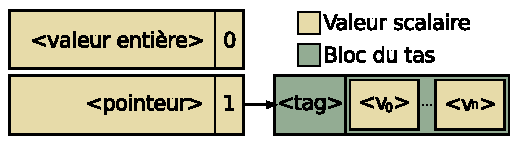
\includegraphics{media/ocaml_value}
\caption{Forme des valeurs}
\end{figure}

\begin{figure}
\centering
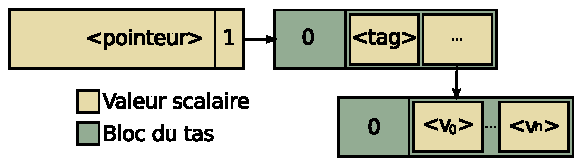
\includegraphics{media/ocaml_variant}
\caption{Forme des variants polymorphes}
\end{figure}

\section{Séparer extraction et analyse d'un \emph{tag}}

La principale contribution réside entre la séparation du calcul d'un tag et du
branchement qui s'ensuivra.

\paragraph{Filtrage de motif} Traditionnellement dans les langages ML, le
\emph{filtrage de motif} est utilisé pour permettre de manière sûre et efficace
la sélection de différentes branches de code.

Les constructeurs d'un type algébrique deviennent chacun une branche. Dans
chaque branche, des noms liés aux paramètres du constructeur testé sont
introduits. Le programmeur n'indique jamais explicitement l'accès aux champs
d'une valeur. Il ne peut même pas nommer un champ en dehors de la branche.

Il est alors simple de vérifier l'exhaustivité du traitement et de garantir
l'absence d'accès à des valeurs inexistantes lors de l'exécution. Enfin le
compilateur se voit offrir beaucoup de libertés pour générer du code efficace
\todo{cite Lefessant, Maranget, … compilation pattern matching}.

\paragraph{Motifs compilés} Le compilateur OCaml choisit de compiler ces motifs
très tôt. Dans le langage \emph{Lambda} il n'existe déjà plus que deux formes
de tests, les \emph{switch} et \emph{if} que l'on retrouve dans les langages
impératifs classiques. Une forme spécialisée de branchement proche du
\emph{goto} est aussi proposée pour factoriser le code des branches.

Les filtrages de haut-niveau sont ainsi traduits via des arbres de décisions,
au travers d'une suite de tests et de tables de sauts.  Le lien entre la
sélection d'une branche et les hypothèses qui y ont amené disparaît -- le
compilateur ne peut que suivre les instructions de projection sous l'hypothèse
que le code traduit est correct.
